% !TEX root =  ../main_manuscript.tex 
\section{Patients and Methods}
\label{c5:sec:pat_methods}
\subsection{Study Cohort}
\label{subsec:cohort}
For developing a statistical model to predict upgrading-risk, we used the world's largest AS dataset, Prostate Cancer International Active Surveillance or PRIAS~\citep{bul2013active}, dated April 2019 (Table~\ref{table:prias_summary}). In PRIAS, biopsies were scheduled at year one, four, seven, ten, and additional yearly biopsies were scheduled when PSA doubling time was between zero and ten years. We selected all 7813~patients who had Gleason grade group~1 at inclusion in AS. Our primary event of interest is an increase in this Gleason grade group observed upon repeat biopsy, called \textit{upgrading} (1134~patients). Upgrading is a trigger for treatment advice in PRIAS. Some examples of treatment options in active surveillance are radical prostatectomy, brachytherapy, definitive radiation therapy, and other alternative local treatments such as cryosurgery, High Intensity Focused Ultrasound, and External Beam Radiation Therapy. Comprehensive details on treatment options and their side effects are available in EAU-ESTRO-SIOG guidelines on prostate cancer~\citep{mottet2017eau}. In PRIAS 2250 patients were provided treatment based on their PSA, the number of biopsy cores with cancer, or anxiety/other reasons. However, our reasons for focusing solely on upgrading are that upgrading is strongly associated with cancer-related outcomes, and other treatment triggers vary between cohorts~\citep{nieboer2018active}.

For externally validating our model's predictions, we selected the following largest (by the number of repeated measurements) six cohorts from Movember Foundation's GAP3 database~\citep{gap3_2018} version~3.1, covering nearly 73\% of the GAP3 patients: the University of Toronto AS (Toronto), Johns Hopkins AS (Hopkins), Memorial Sloan Kettering Cancer Center AS (MSKCC), King's College London AS (KCL), Michigan Urological Surgery Improvement Collaborative AS (MUSIC), and University of California San Francisco AS (UCSF, version~3.2). Only patients with a Gleason grade group~1 at the time of inclusion in these cohorts were selected. Summary statistics are presented in Section~\ref{c5:appendix:full_results}.

\begin{table}
\small
\centering
\caption{\textbf{Summary of the PRIAS dataset as of April 2019}. The primary event of interest is upgrading, that is, increase in Gleason grade group from group~1~\citep{epsteinGG2014} to 2 or higher. IQR:~interquartile range, PSA:~prostate-specific antigen. Study protocol URL: \url{https://www.prias-project.org}}
\label{table:prias_summary}
\begin{tabular}{lr}
\toprule
\textbf{Characteristic} & \textbf{Value}\\
\midrule
%Total centers & $> 100$\\
Total patients & 7813\\
Upgrading (primary event) & 1134\\
Treatment & 2250\\
Watchful waiting & 334\\
Loss to follow-up & 249\\
Death (unrelated to prostate cancer) & 95\\
Death (related to prostate cancer) & 2\\
\midrule
Median age at diagnosis (years) & 66 (IQR: 61--71)\\
Median maximum follow-up per patient (years) &  1.8 (IQR: 0.9--4.0)\\
Total PSA measurements & 67578\\
Median number of PSA measurements per patient &  6 (IQR: 4--12)\\
Median PSA value (ng/mL) & 5.7 (IQR: 4.1--7.7)\\
Total biopsies & 15686\\
Median number of biopsies per patient &  2 (IQR: 1--2)\\
\bottomrule
\end{tabular}
\end{table}

\paragraph{Choice of predictors:} In our model, we used all repeated PSA measurements, the timing of the previous biopsy and Gleason grade, and age at inclusion in AS. Other predictors such as prostate volume, MRI results can also be important. MRI is utilized already for targeting biopsies, but regarding its use in deciding the time of biopsies, there are arguments both for and against it~\citep{kasivisvanathan2020magnetic,chesnut2019role,schoots2015magnetic}. MRI is still a recent addition in most AS protocols. Consequently, repeated MRI data is very sparsely available in both PRIAS and GAP3 databases to make a stable prediction model. Prostate volume data is also sparsely available, especially in validation cohorts. Based on these reasons, we did not include them in our model. However, the model we propose next is extendable to include MRI and other novel biomarkers in the future.

% !TEX root =  ../main_manuscript.tex 
\subsection{Statistical Model}
Modeling an AS dataset such as PRIAS, posed certain challenges. First, PSA was measured longitudinally, and over follow-up time it did not always increase linearly. Consequently, we expect that PSA measurements of a patient are more similar to each other than of another patient. In other words, we need to accommodate the within-patient correlation for PSA. Second, PSA was available only until a patient observed upgrading. Thus, we also need to model the association between the Gleason grades and PSA profiles of a patient, and handle missing PSA measurements after a patient experienced upgrading. Third, since the PRIAS biopsy schedule uses PSA, a patient's observed time of upgrading was also dependent on their PSA. Thus, the effect of PSA on the upgrading-risk need to be adjusted for the effect of PSA on the biopsy schedule. Fourth, many patients obtained treatment and watchful waiting before observing upgrading. Since we considered events other than upgrading as censoring, the model needs to account for patients' reasons for treatment or watchful waiting (e.g., age, treatment based on observed data). A model that handles these challenges in a statistically sound manner is the joint model for time-to-event and longitudinal data~\citep{tomer2019,coley2017prediction,rizopoulos2012joint}.

Our joint model consisted of two sub-models. Namely, a linear mixed-effects sub-model~\citep{laird1982random} for longitudinally measured PSA (log-transformed), and a relative-risk sub-model (similar to the Cox model) for the interval-censored time of upgrading. Patient age was used in both sub-models. Results and timing of the previous negative biopsies were used only in the risk sub-model. To account for PSA fluctuations~\citep{nixon1997biological}, we assumed t-distributed PSA measurement errors. The correlation between PSA measurements of the same patient was established using patient-specific random-effects. We fitted a unique curve to the PSA measurements of each patient (Panel~A, Figure~\ref{c5:fig:3}). Subsequently, we calculated the mathematical derivative of the patient's fitted PSA profile~(\ref{c5:eq:rel_risk_model}), to obtain his follow-up time specific instantaneous PSA velocity (Panel~B, Figure~\ref{c5:fig:3}). This instantaneous velocity is a stronger predictor of upgrading than the widely used average PSA velocity~\citep{cooperberg2018refined}. We modeled the impact of PSA on upgrading-risk by employing fitted PSA value and instantaneous velocity as predictors in the risk sub-model (Panel~C, Figure~\ref{c5:fig:3}). We adjusted the effect of PSA on upgrading-risk for the PSA dependent PRIAS biopsy schedule by estimating parameters using a full likelihood method (proof in Chapter~\ref{c2:appendix:B}). This approach also accommodates watchful waiting and treatment protocols that are also based on patient data. Specifically, the parameters (Section~\ref{c5:appendix:model_specification}) of our two sub-models were estimated jointly under the Bayesian paradigm using the R package \textbf{JMbayes}~\citep{rizopoulosJMbayes}.

\begin{figure}
\centerline{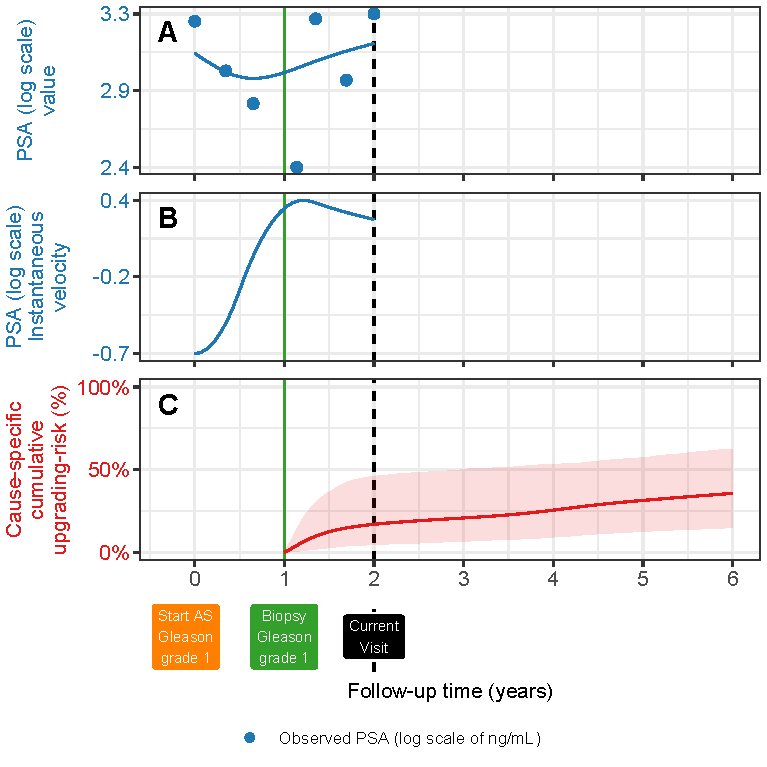
\includegraphics{contents/c5/images/c5_fig3.pdf}}
\caption{\textbf{Illustration of the joint model on a real PRIAS patient}. \textbf{Panel~A:} Observed PSA (blue dots) and fitted PSA (solid blue line), log-transformed from ng/mL. \textbf{Panel~B:} Estimated instantaneous velocity of PSA (log-transformed). \textbf{Panel~C}: Predicted cause-specific cumulative upgrading-risk (95\% credible interval shaded). Upgrading is defined as an increase in the Gleason grade group from group~1~\citep{epsteinGG2014} to 2 or higher. This upgrading-risk is calculated starting from the time of the latest negative biopsy (vertical green line at year one of follow-up). The joint model estimated it by combining the fitted PSA (log scale) value and instantaneous velocity, and time of the latest negative biopsy. Black dashed line at year two denotes the time of current visit.}
\label{c5:fig:3}
\end{figure}

\subsection{Risk Prediction and Model Validation}
Our model provides predictions for upgrading-risk over the entire future follow-up period of a patient (Panel~C, Figure~\ref{c5:fig:3}). However, we recommend using predictions only after year one. This is because most AS programs recommend a confirmatory biopsy at year one, especially to detect patients who may be misdiagnosed as low-grade at inclusion in AS. The model also automatically updates risk-predictions over follow-up as more patient data becomes available (Figure~\ref{c4:fig:2}). We validated our model internally in the PRIAS cohort, and externally in the largest six GAP3 database cohorts. We employed calibration plots~\citep{royston2013external,steyerberg2010assessing} and follow-up \textit{time-dependent} mean absolute risk prediction error or MAPE~\citep{rizopoulos2017dynamic} to graphically and quantitatively evaluate our model's risk prediction accuracy, respectively. We assessed our model's ability to discriminate between patients who experience/do not experience upgrading via the time-dependent area under the receiver operating characteristic curve or AUC~\citep{rizopoulos2017dynamic}. 

The aforementioned \textit{time-dependent} AUC and MAPE~\citep{rizopoulos2017dynamic} are temporal extensions of their standard versions~\citep{steyerberg2010assessing} in a longitudinal setting. Specifically, at every six months of follow-up, we calculated a unique AUC and MAPE for predicting upgrading-risk in the subsequent one year (Appendix~\ref{c5:appendix:validation}). For emulating a realistic situation, we calculated the AUC and MAPE at each follow-up using only the validation data available until that follow-up. Last, to resolve any potential model miscalibration in validation cohorts, we aimed to recalibrate our model's baseline hazard of upgrading (Appendix~\ref{c5:appendix:validation}), individually for each cohort.